% !TeX root = ..\..\main.tex
\chapter{Introduction}
\pagenumbering{arabic}
This report studies a vital financial derivative in today's markets, namely options. The importance of the option market has been shown by empirical studies which suggest that option trading improves information efficiency in the broader stock market~\cite{PanInfoEffic,li2021effect}, and also that firms with listed options experience lower implied cost of equity capital~\cite{naikerLowEquity}; indicating that options trading reduces the cost of capital~\cite{li2021effect}. The popularity of the options market can easily be seen in \autoref{C1fig:OptionVolume}, which shows the exponential growth in trading volume since standardized, exchange-traded stock options were first listed in The Chicago Board Options Exchange in 1973~\cite{markham2002financial}. In 2020 single stock option trading volume became higher than the underlying stock volume for the first time ever~\cite{yahooOptions}. 
\nline{}
It is this explosive popularity and significance which have motivated this report. 
\\\\
We will begin by describing standard options and explore popular methods that are used to price them. We will then move onto Asian options and look at the literature surrounding how to price them before implementing several pricing methods with the use of \textsc{Matlab}. Furthermore, we will then take an analytical approach to determine how Asian options can be priced accurately and efficiently.
\\\\

\begin{figure}[H]
    \centering
    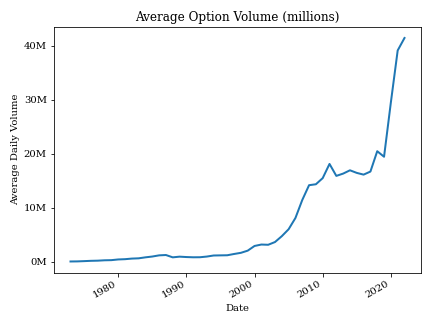
\includegraphics[width=\sOneSize\textwidth]{Chapters/C1/plots/OptionVolume.png}
    \caption{Time series plot of the average daily option trading volume per annum. Data from by the Options Clearing Corporation (OCC)~\cite{THEOCC}. Source code: \autoref{ApPy:lst option volume plot}}\label{C1fig:SymRw}
\end{figure}

\section{A brief overview of call and put options}

Options are a particular type of financial derivative, a contract that details the conditions under which payments are made between two counterparties. They are purchased for a set fee, and in return the buyer is granted the right, but not the obligation to buy or sell an underlying asset --- such as commodities, stocks or bonds --- for a predetermined price (the strike price) on or before a determined date (the expiry date).
\nline{}
Call options allow the buyer to purchase an asset for the strike price at a future date. The buyer can make a return if the value of the asset is worth more than the strike price when exercised. Alternatively, put options allow the buyer to sell an asset for the strike price at a future date and the buyer can make a return if the value of the asset is less than the strike price when exercised.
\nline{}
The option market is widely considered a venue for informed trading~\cite{li2021effect,hu2014,chak2004}, that is, investors trading with superior knowledge of the probability distribution of share prices, through either access to private information or skilful processing of public information~\cite{grossman1975application}. 

\subsection{A short history of option trading}
The history of financial options can be traced as far back as 6th century BCE when ancient Greek mathematician and philosopher Thales of Miletus predicted through his astrological knowledge there was going to be a great olive harvest. As he did not have much money, he used what he had as a deposit on the rights to the local olive presses; due to no competition he secured this at a relatively low price. When the harvest proved to be bountiful leading to high demand, Thales charged a high price for use of the presses and reaped a considerable profit. His deposit gave him the right but not the obligation to hire the presses, thus his losses were limited to his initial deposit~\cite{OptionFirst, 1877aristotle}.
\nline{}
Whilst this is quite a positive look on option trading, throughout history this has not always been the case. During the Dutch tulip bubble of the seventeenth century, tulips were seen as a status symbols which caused high demand and consequently drove their prices up, creating a bubble~\cite{dash2011tulipomania}. Tulip growers would buy puts to protect their profits in case the price of tulip bulbs went down and wholesalers would buy calls to protect against the risk of tulip bulbs going up. When the bubble eventually burst, there was no way to force investors to fulfil their obligations of the options contracts, due to the unregulated nature of the option market. This ultimately led to options gaining a dubious reputation and bans were later placed on them within Britain between 1733--1860~\cite{OptionBan}. 
\nline{}
During the late nineteenth century, brokers started to arrange deals between buyers and sellers of options for particular stocks at prices that were arranged between the two parties. Trades were arranged similarly until the 1960s when the options market started to become regulated by the Chicago Board of Trade. In 1973, the Chicago Board of Options Exchange (CBOE) began trading and for the first time options contracts were properly standardized. At the same time, the Options Clearing Corporation was established for centralized clearing and enforcing the proper fulfilment of contracts, ensuring that they were honoured~\cite{markham2002financial}.

\subsection{Standard options}

A standard option comes in two styles; European: which restricts the holder of the option to only exercise the option on the expiry date, and American: which allows the holder to exercise the option at anytime up till or on the expiry date. They will take the current value of the underlying asset as the spot price --- that is the price that the asset can be purchased for on the open market. The payoff in this case then becomes the difference between the spot price and strike price.

\subsection{Asian options}

Whilst standard options involve using the spot price as the underlying value of the asset; this is not always the case with so-called exotic options. Exotic options differ in their payment structures, expiration dates, and/or strike prices. In the case of exotic fixed-strike price Asian options, the average price of the asset is used in place of the underlying asset value. This differs from fixed-price Asian options which instead use the average price of the asset to take place of the strike price. These are the two main variations of Asian style options but both of these can be varied further in how the averaging is calculated, for example: geometrically, arithmetically, average taken every day or average taken at the start of each month and so on. They can be varied further by having an expiry structure matching a European or American style option.

\section{Market definition and assumptions}

To begin pricing options we must first establish assumptions on the value of assets and the market in which they are traded. We will consider a market in which there are two classes of assets; risk-free assets and risky assets. We allow derivatives to exist on risky assets.

\subsection{Asset definitions}

We define our two classes of assets with the following assumptions:

\subsubsection{Risk-free assets}

Risk-free assets are assumed to have no uncertainty in regard to their future value and defined as returning interest continuously compounded at a fixed rate \(r\). Hence, an investment of \(A\) made at time \(t\) will return \(A^{r\left(T-t\right)}\) at time \(T>t\) with no uncertainty. These can be positive e.g., making an investment, or negative e.g., taking out a loan. Risk-free assets are akin to fixed rate investments at a well-know bank or government bonds. However, even sovereign nations have been known to default on their bond repayments so in reality are not truly risk-free, but instead considered low-risk~\cite{kitanov2015risk}.

\subsubsection{Risky assets}

Risky assets are assets in which the future value can not be determined without at least some uncertainty. These are typically shares in a company or commodities such as gold and oil. These assets are traded on the open market and their value is heavily dependent on the balance of supply and demand of the asset; this in turn is dependent on so many variables that we assume their future value to be a random process. Depending on our model we can make different assumptions on the distribution of this process and thus how the value evolves over a time period. In practice has been arguments made for the future value of risky assets are truly random~\cite{RandomWalkFama}, and other arguments that propose they are instead at least partly deterministic where patterns and trends exists~\cite{shiller}.

\subsection{Market Assumptions}

We shall assume that an investor may hold any quantity (including negative and/or fractional) of an asset, known as the \textit{divisibility} and \textit{short-selling} assumption. We will also assume that our market is \textit{frictionless} --- that is that any quantity of assets can be bought and sold at the same price with no transaction cost and are entirely \textit{liquid} meaning there is always a buyer for every seller and vice versa.
\nline{}
In practice these assumptions do not accurately represent real markets, for example it is common place for markets to have bid-ask spreads which represents the different in price at which you can buy and sell assets for. Furthermore, transaction costs are impossible to fully eliminate --- even in scenarios with no tax or commission fees, buying or selling assets (especially in large quantities) will in theory have an effect on the supply and demand of that asset; this introduces market impact costs~\cite{moro2009market}. There are other transaction fees to also consider such as: time spent deciding what assets to buy, computing power costs and their associated opportunity costs.

\subsubsection{No-Arbitrage assumption}

Perhaps our most important market assumption is the No-Arbitrage principle; sometimes referred to as the no free-lunch principle. This assumption states that there can be no risk-free way to get a better rate of return than the market risk-free interest rate, \(r\). The logic behind this assumption is that if there exists a way to earn a higher rate of return than \(r\) with no initial outlay; than other traders would employ the same method and market forces would eliminate the arbitrage opportunity. This assumption assumes that markets are perfectly efficient meaning all traders have access to the same information and that market adjustments to supply and demand happen instantaneously, which we know not to be true in practice.

\section{Asset pricing models}

Having now established our market assumptions, we must now define our assumptions on the random process which describes how the asset value may evolve over a specified time period. We will first introduce the mathematical concepts in which these models are built upon. Then we will introduce a simple asset model and one which has more assumptions in hopes of better describing the future asset value in practice.

\subsubsection{Stochastic processes}

A stochastic process is defined as a collection of random variables defined on a common probability space \( (\Omega ,\mathcal{F},P) \), where \( \Omega \)  is a sample space, \( \mathcal{F} \) is a \( \sigma \)-algebra, and \( P \) is a probability measure; and the random variables, indexed by some set \( T \), all take values in the same mathematical space \(S\), which must be measurable with respect to some \( \sigma \)-algebra \( \Sigma \)~\cite{lamperti1977stochastic}.
\nline{}
A discrete stochastic process is a sequence of random variables which represent observations taken at discrete times from a random system, e.g.\ observations \( \{X_i\,:\, i \in \nat_{[0,n]}\} \) at times \( t = t_0,t_1,\,\dots \,t_n \). We can let our market be the random system and our observations, \( X_i \) be the value of our asset observed on the \( i^\text{th}\) day. This is a typical example of structuring an asset market as a discrete stochastic process; we will later see how this is helpful for building our asset pricing models.

\subsubsection{Markov Process}

Maybe insert a little bit of text explaining markov processes, add to brownian motion section that it is a form of markov process.

\subsubsection{Brownian Motion (Wiener Process)}

Brownian motion is a pattern of motion first described by the botanist Robert Brown in 1827 when observing the unpredictable motion of pollen of a plant through a microscope~\cite{pearle2010brown}. The motion typically consists of random fluctuations in a particle's position inside a subdomain, followed by relocation to another subdomain. This motion has applications in many fields of study such as pure and applied mathematics, economics and physics. In statistics, Brownian motion is described by the Wiener Process.
\nline{}
A Wiener process, \( \wei_t \) is a continuous-time stochastic process named after Norbert Wiener for his study into the mathematical properties of one-dimension Brownian motion~\cite{wiener1976norbert}; it is characterized by the following properties~\cite{durrett2019probability}:

\begin{enumerate}
    \item \( \wei_0 \) = 0
    \item \( \wei \) has independent increments, i.e. \( \forall t>0 \), the future increments \( \wei_{t+u} - \wei_t, u \geq 0 \), are independent of the past values \( \wei_s, s \leq t \).
    \item\label{Weiner process Gaussian increments} \( \wei \) has Gaussian increments: \( \wei_{t+u} - \wei_t \) is normally distributed with mean 0 and variance \( u \), i.e. \hfill\break{} \( \wei_{t+u} - \wei_t \sim \norm\p{0, u}\).
    \item \( \wei \) has continuous paths: \( \wei_t \) is continuous in \( t \).
\end{enumerate}

\subsubsection{Asset Prices as Brownian Motion}

The French mathematician Louis Bachelier is often attributed to pioneering using Brownian motion to model asset prices when he did so in his PhD thesis “The Theory of Speculation'' (1900)~\cite{Bachelier+2007}. However, a lesser known French economist Jules Renault was first to do so in his 1863 publication “calcul des chances et philosophie de la bourse''~\cite{RegnaultFirst}.
\nline{}
Regnault hypothesized that asset prices change according to a game of ``heads or tails'':
\begin{quotation}
    ``On the stock market, the whole mechanism of the game comes down to two opposite possibilities: increasing and decreasing. Each one can always appear with an equal facility'' \hfill{}\nolinebreak\cite{regnault1863calcul,RegnaultFirst}
\end{quotation}
He also claimed ``the deviation of prices is directly proportional to the square root of time'' this is a result we would expect to see from a Weiner process (\autoref{Weiner process Gaussian increments}). Fast-forward to 1900 and Bachelier further developed the theory of asset prices moving according to a random process; his ideas depended on markets being efficient. Bachelier theorized in his thesis that as soon as prices becomes predictable, it immediately becomes exploited. However, he believed all traders to have access to all available information which leads to these predictable patterns instantly disappearing. Bachelier believed prices took what we now call ``random walks'' above and below their true value, as competing traders attempt to beat the market. He would go on to conduct a study on French government bonds, concluding that their price changes were consistent with a random walk model; furthermore, Bachelier would formulate many of the mathematical properties of the stochastic process now known as Brownian motion~\cite{Bachelier+2007}.
\nline{}
These contributions by Bachelier went largely unnoticed until the mid 20th century when several historic publications formalized and furthered the theory surrounding the Random-Walk and Efficient-Market Hypothesis~\cite{Maurice_Kendall_RandomWalk, cootner1964random, RandomWalkFama}. These hypotheses were heavily studied throughout the 20th century and pathed the way for many advances in mathematical finance. Over the decades there has been mixed evidence to support the hypothesis that markets can not be predicted. More recently studies have shown that market predictability has become more difficult due to advances in trading technology and investor learning~\cite{welch2008comprehensive,mclean2016does}. However, for our market and asset assumptions, and our ultimate goal of implementing pricing models for financial options; random walk and Brownian motion models are sufficient.
\subsection{Random-walk model}\label{subsec: RW model}

\begin{figure}[]
    \centering
    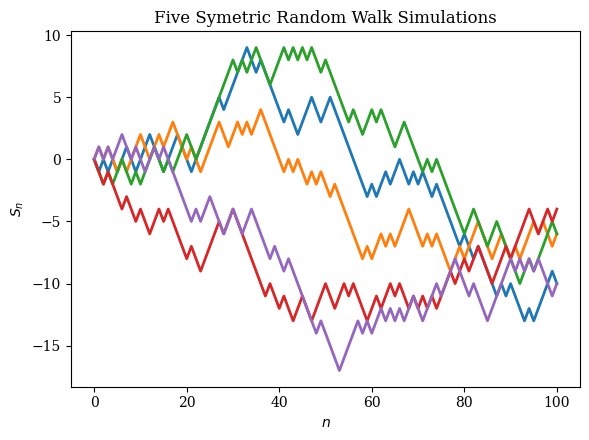
\includegraphics[width=\sOneSize\textwidth]{Chapters/C1/plots/RW_Simulations.png}
    \caption{Five simulations of a symmetric random walk with probability \(p = 0.5\) and no drift. Source code: \autoref{ApPy:SymRW}}\label{C1fig:OptionVolume}
\end{figure}

A random walk is a type of stochastic process that describes a path in which at every movement forward in time the movement in space is decided by a random process. A simple 2 dimension case for example; we construct a path in which we start at 0 and for every time step forward, we flip a fair coin to decide if we move up or down. We let \( S_i \) be our position of the path at time \( t = t_i \) and \(y_i\) be the result of our \( i^\text{th} \) coin toss and \( Y_i \) be how the toss effects our path; where \( Y_i = 1 \) if \( y_i = \text{heads} \) and \(Y_i = -1\) if \( y_i = \text{tails} \). This random walk is called symmetric as it goes up or down by the same amount. If we were to plot our path it would look something like:

\subsubsection{The general case}

It follows that we can construct a random walk for the general case where we may change the probabilities, the size of the step taken and also introduce a drift parameter. This is written as follows:

\begin{align*}
    S_0 &= S_0 \\
    S_n &= S_{n-1} + \mu + \sigma Y_i
\end{align*}

Where \(\mu \) is the drift, \(\sigma \) scales the movement and \(Y_i\) are identically and independently distributed (i.d.d.):

\begin{equation*}
    Y_i = 
    \begin{cases}
       \alpha& \quad \text{with } P(Y_i = \alpha) = p; \\
       \beta& \quad \text{with } P(Y_i = \beta) = (1-p)
    \end{cases}
\end{equation*}

We let \(S_i \) be the price of an asset on the \(i^{\text{th}}\) day, thus \(S_0\) is the current price of the asset. The drift in terms of an asset model allows us to model in the expected increase/decrease in price of the asset, where scale allows us to model the volatility (the magnitude of movements). There are different methods in which we could employ to calculate our drift and scale parameters, this will typically involve using historical data but can extend to take into account speculation about the underlying asset.

\subsubsection{Drawbacks of a random walk to model asset prices}

We can begin to see how this path may reflect the price an asset which future value is determined by a random event. However, this model comes with several drawbacks: This model only permits the price of the asset to go up and down by a fixed amount, further to this point, the amount is detached from the current value of the asset; we may instead expect that the value change would be proportional to the current value. Lastly, the random walk model also allows asset prices to go negative which typically is considered impossible. However, during April 2020, oil futures became sharply negative for the first time in history~\cite{NegativeOil}. This has lead to people to reconsider the random walk model and see this instead as a positive in specific circumstances. An alternative approach instead applies the random walk model to rate of return instead of asset value, which of course can often be negative.

\subsection{Geometric Brownian model}

A better alternative is the geometric Brownian model, shown in \autoref{eqn: Geo Brownian Motion}. This model addresses the drawbacks of the simple random walk model. First, we can see that the left-hand side of the equation is the percentage increase from the previous time to the current time. This means our price change is not detached from the previous value and the absolute value can never become negative.
\nline{}
We introduce a new term, \(\delta t\), this is taken to be a fixed time interval which is comparatively small to the time interval \(t \in [0,T]\); where \(t = T\) is the final time of the model. We now let the price of the asset, \(S_i = S(i)\) no longer be measured on the \(i^{\text{th}}\) day, but instead the \(i^{\text{th}}\) number of the time interval \(\delta t\). It is common to calculate \(\delta t\) by considering your entire time range, \(t\in[0,T]\) and splitting this range into \(N\) \(\delta t\) increments, where \(N\) is some large number; hence \(S_{N} = S\p{N\delta t = T} = S_T\). Now, if we were to consider a drift parameter \(\mu \) which represents the expected price increase in one unit of time, it would follow that the increase over our time increment \(\delta t\) would be \(\delta t \mu \). The variance (volatility) of the percentage increase at the final, \(N^{\text{th}}\) step would be \(N\) times the variance at each time interval step, so we would expect this variance to be proportional to \(\delta t\).

\begin{equation}\label{eqn: Geo Brownian Motion}
    \frac{S_{n+1} - S_n}{S_n} = \delta t\mu + \sqrt{\delta t}\sigma Y_{n+1}
\end{equation}

\section{Pricing options}

Since the holder of the contract is not obliged to exercise the contract at the expiry time, they do not hold any liability in the absence of a price to purchase the option. The problem then becomes, what is the correct price to charge the holder of the option to balance this inequality of liability.



\subsection{Pricing standard options}

\subsubsection{Binomial method}

\subsubsection{Black-Scholes Formula}

\subsection{Pricing Asian options}

\subsubsection{Hull-White model}

\subsubsection{Costabile adjusted binomial method}

\subsubsection{Analytical solution for geometric average Asian options}

\subsection{Monte-Carlo method}=